\documentclass{beamer}

\mode<presentation> {

%\usetheme{default}
%\usetheme{AnnArbor}
%\usetheme{Antibes}
%\usetheme{Bergen}
%\usetheme{Berkeley}
%\usetheme{Berlin}
%\usetheme{Boadilla}
%\usetheme{CambridgeUS}
%\usetheme{Copenhagen}
%\usetheme{Darmstadt}
%\usetheme{Dresden}
%\usetheme{Frankfurt}
%\usetheme{Goettingen}
%\usetheme{Hannover}
%\usetheme{Ilmenau}
%\usetheme{JuanLesPins}
%\usetheme{Luebeck}
%\usetheme{Madrid}
%\usetheme{Malmoe}
%\usetheme{Marburg}
%\usetheme{Montpellier}
%\usetheme{PaloAlto}
%\usetheme{Pittsburgh}
%\usetheme{Rochester}
%\usetheme{Singapore}
%\usetheme{Szeged}
%\usetheme{Warsaw}
\usetheme{Aalto}

%\usecolortheme{albatross}
%\usecolortheme{beaver}
%\usecolortheme{beetle}
%\usecolortheme{crane}
%\usecolortheme{dolphin}
%\usecolortheme{dove}
%\usecolortheme{fly}
%\usecolortheme{lily}
%\usecolortheme{orchid}
%\usecolortheme{rose}
%\usecolortheme{seagull}
%\usecolortheme{seahorse}
%\usecolortheme{whale}
%\usecolortheme{wolverine}

%\setbeamertemplate{footline}
%\setbeamertemplate{footline}[page number]

%\setbeamertemplate{navigation symbols}{}
}

\usepackage{graphicx}
\usepackage{booktabs}
\usepackage{amsmath}

\title{ELFI: Engine for Likelihood Free Inference}

\author{Antti Kangasr\"a\"asi\"o}
\institute[Probabilistic Machine Learning Group]
{
Aalto University, Probabilistic Machine Learning Research Group\\
\medskip
Joint work with:
Jarno Lintusaari (Aalto),
Henri Vuollekoski (Aalto),
Kusti Skyt\'en (Aalto),
Marko J\"arvenp\"a\"a (Aalto),
Michael Gutmann (University of Edinburgh),
Aki Vehtari (Aalto),
Jukka Corander (University of Oslo),
Samuel Kaski (Aalto)
}
\date{July 25th, 2017}

\begin{document}

\begin{frame}
\titlepage
\end{frame}

\begin{frame}
\frametitle{Overview}
\tableofcontents
\end{frame}

%------------------------------------------------
\section{Approximate Bayesian Computation}
%------------------------------------------------

\subsection{What is ABC}

\begin{frame}
\frametitle{Likelihood function}
Likelihood function is central in model-based inference\\
\medskip
In many cases, inference consists of just finding the maximum of the likelihood function (ML point estimate)\\
\medskip
However, with many complex models either:
\begin{itemize}
\item No explicit likelihood function exists
\item Evaluating the likelihood function is infeasible
\end{itemize}
\medskip
Examples include:
\begin{itemize}
\item Climate models
\item Biological models
\item Cognitive models
\end{itemize}
\end{frame}

\begin{frame}
\frametitle{What is Approximate Bayesian Computation}
ABC is a set of inference methods that bypass the evaluation of the likelihood function\\
\medskip
The core idea is to repeatedly simulate predictions from the model and evaluate their discrepancy with the observation data\\
\medskip
\textbf{Intuition:} If parameters lead to predictions that match with the observation data, then these parameters have high likelihood\\
\medskip
ABC methods are based on Bayesian statistics, and with some assumptions we can closely approximate the true likelihood
\end{frame}

\begin{frame}
\frametitle{ABC Visual Demonstration}
\vspace{-1em}
\begin{figure}[ht]
\centerline{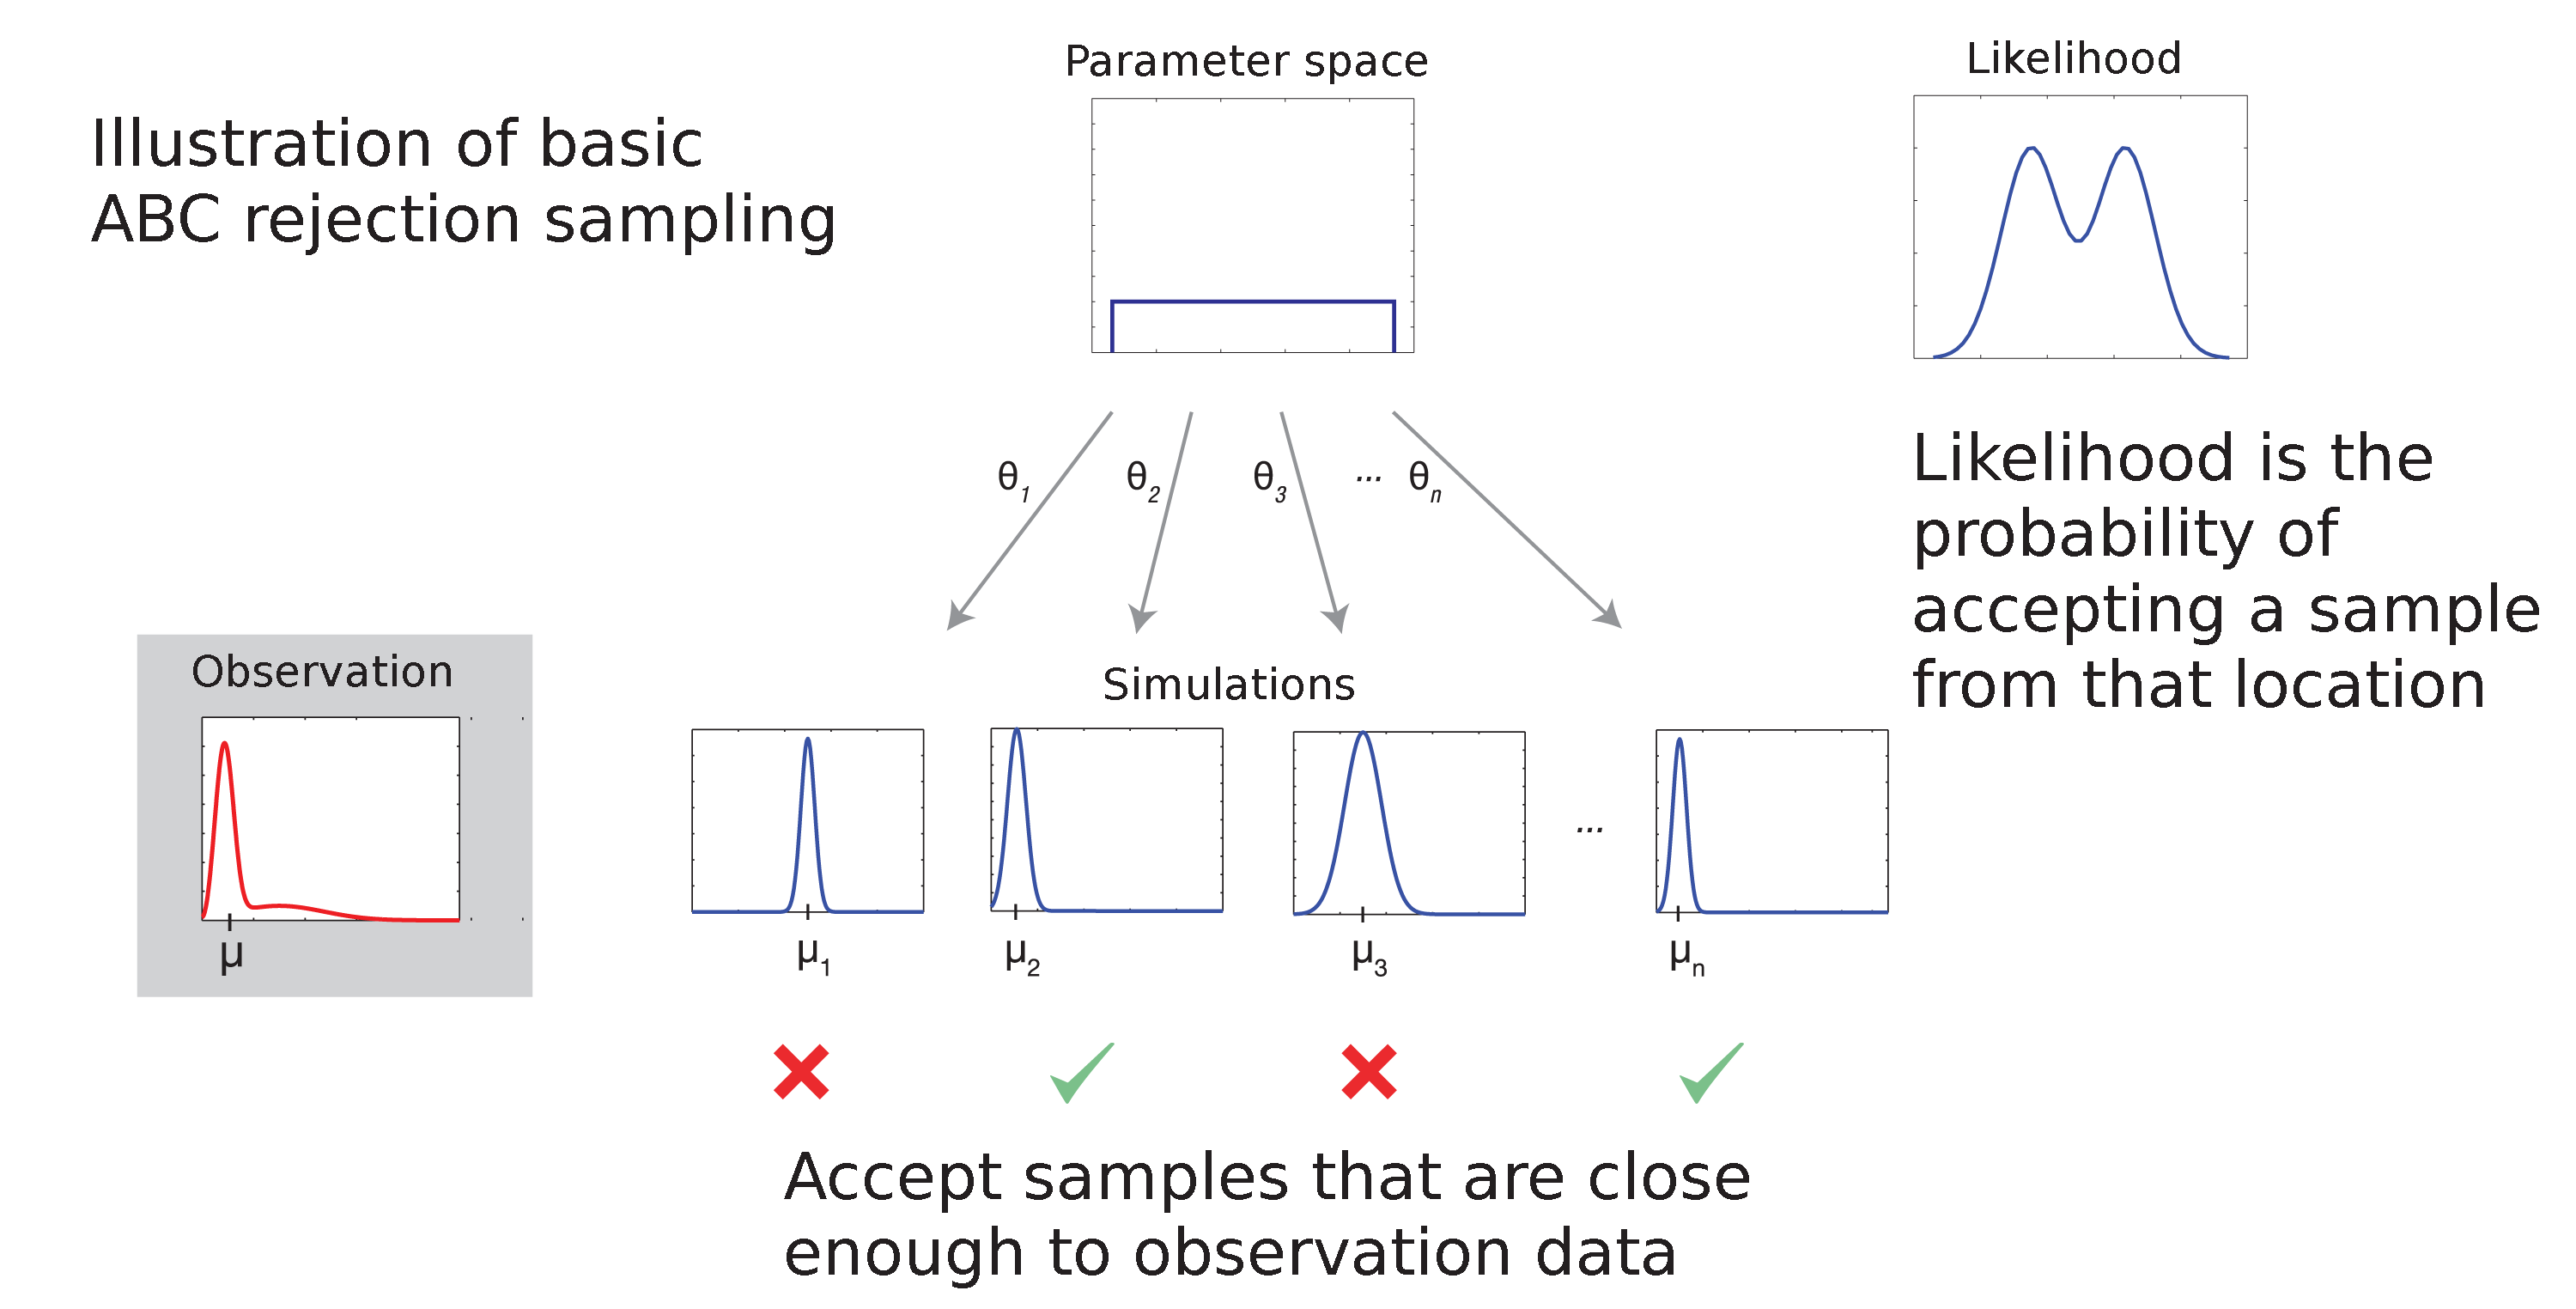
\includegraphics[width=\columnwidth]{img/abc1.png}}
\end{figure}
\vspace{-1em}
\tiny{Figure adapted from: Sunnaker et al., ABC, 2013, \url{https://doi.org/10.1371/journal.pcbi.1002803}}
\end{frame}

\subsection{Why use ABC}

\begin{frame}
\frametitle{Why use ABC}
\end{frame}

\subsection{Examples of ABC}

\begin{frame}
\frametitle{Examples of ABC}
\end{frame}

%------------------------------------------------
\section{ELFI Python Library}
%------------------------------------------------

\subsection{What is ELFI}

\begin{frame}
\frametitle{What is ELFI}
\end{frame}

\subsection{What features does ELFI have}

\begin{frame}
\frametitle{What features does ELFI have}
\end{frame}

\subsection{Demonstration}

\begin{frame}
\frametitle{Demonstration}
\end{frame}

\end{document}
